\documentclass[11pt,a4paper]{article}

% ===== Packages =====
\usepackage[utf8]{inputenc}
\usepackage[T1]{fontenc}
\usepackage{amsmath,amssymb,amsfonts}
\usepackage{graphicx}
\usepackage{booktabs}
\usepackage{hyperref}
\usepackage[numbers,sort&compress]{natbib}
\usepackage{xcolor}
\usepackage{algorithm}
\usepackage{algpseudocode}
\usepackage{subcaption}
\usepackage{siunitx}
\usepackage{adjustbox}
\usepackage{soul}
\usepackage{tikz}
\usetikzlibrary{arrows.meta, positioning, shapes, calc}
\usepackage{longtable}
\usepackage[dvipsnames]{xcolor}
\usepackage[margin=1in]{geometry}
\usepackage{lineno}  % For line numbers during review

% ===== Hyperref Setup =====
\hypersetup{
    colorlinks=true,
    linkcolor=blue,
    citecolor=blue,
    urlcolor=blue
}

% ===== Custom Commands =====
\newcommand{\vect}[1]{\mathbf{#1}}
\newcommand{\matr}[1]{\mathbf{#1}}

% ===== Title and Authors =====
\title{Sequential RNN Deep Networks for Predicting UV Absorption Properties of Organic Molecules}

% \author{
%     First Author$^{1,*}$, Second Author$^{2}$, Third Author$^{1}$ \\[0.5em]
%     \small $^1$Department of Chemistry, University Name, City, Country \\
%     \small $^2$Department of Computer Science, University Name, City, Country \\[0.3em]
%     \small $^*$Corresponding author: email@university.edu
% }

\author{
    Umesh Arampath$^{1,*}$ \\[0.5em]
    \small $^1$Department of Mathematics, University of Iowa, Iowa City, USA \\
    \small $^1$Midwest Bioprocessing Center, Illinois, USA \\[0.3em]
    \small $^*$Corresponding author: uarampath@mwbioprocessing.com
}

\date{}

\begin{document}

\maketitle

% ===== Abstract =====
\begin{abstract}
Accurate prediction of UV absorption properties is essential for the rational design of molecules 
targeting applications in sunscreen formulation, pharmaceutical development, and optoelectronic 
materials. However, predicting the maximum absorption wavelength ($\lambda_{\max}$) of organic 
molecules remains challenging due to the complex dependence of UV absorption on molecular 
electronic structure and solute--solvent interactions. In this work, we present a deep learning 
framework based on bidirectional Gated Recurrent Unit (BiGRU) networks that predicts 
$\lambda_{\max}$ directly from SMILES string representations of organic molecules. We leverage 
two comprehensive experimental UV/Vis absorption databases---comprising over 38,000 records 
across more than 15,000 unique organic chromophores measured in hundreds of solvent 
conditions to train and evaluate our models. A key contribution of this work is the integration 
of solvent information into the predictive framework through a sequence concatenation strategy, 
where SMILES representations of both the solute and solvent are combined into a single input 
sequence with special delimiter tokens, enabling the model to learn solvent effects 
directly from data. The baseline model trained without solvent information achieved an RMSE of 
24.36~nm, while the solvent-aware model reduced the prediction error to 20.34~nm, representing 
a 16.5\% improvement. Experimental validation against UV-Vis spectroscopy measurements on 
known UV-absorbing compounds including avobenzone, ferulic acid, homosalate, octisalate, and 
oxybenzone demonstrated strong agreement between predicted and experimentally determined 
$\lambda_{\max}$ values, with prediction errors ranging from 5 to 11~nm. These results 
establish sequential RNN architectures with solvent-aware encoding as an effective and 
computationally efficient approach for predicting UV absorption properties of organic 
chromophores.
\end{abstract}

\noindent\textbf{Keywords:} machine learning; molecular design; deep learning; SMILES; property prediction

\section{Introduction}

\begin{figure}[H]
  \centering
  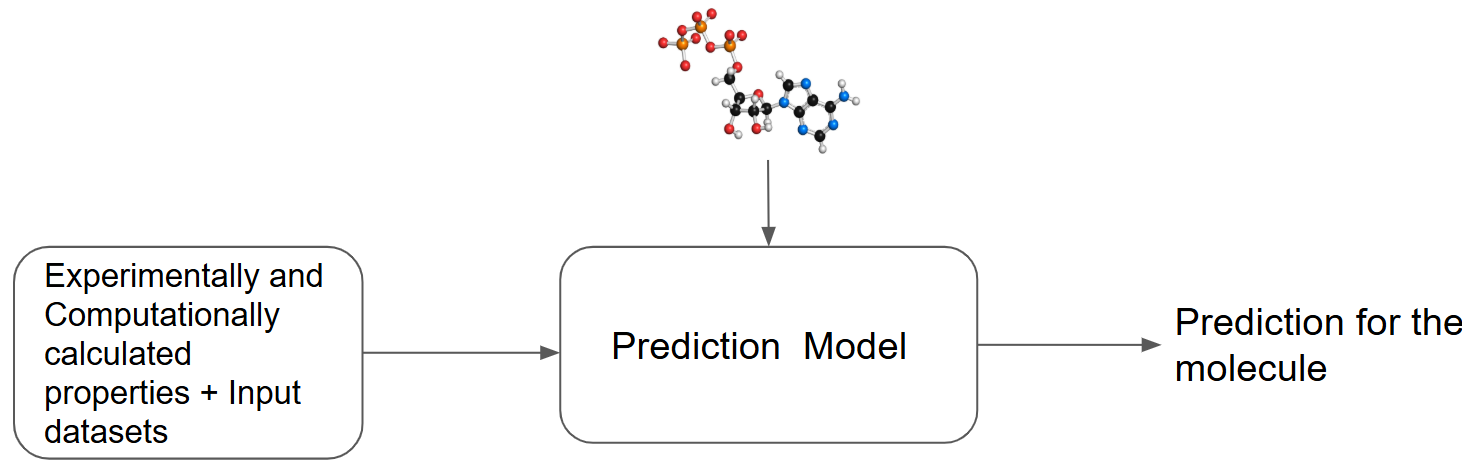
\includegraphics[scale=0.5]{p_1.png}
  \caption{Schematic overview of the predictive modeling process  }
  \label{fig:myfig}
\end{figure}

Molecular property prediction is a fundamental task in computational chemistry and drug discovery, aiming to estimate physicochemical, biological, or pharmacological properties of molecules directly from their structural representations \cite{wuMoleculeNetBenchmarkMolecular2018}. Traditional approaches rely on handcrafted molecular descriptors or fingerprints, which require domain expertise and may not capture all relevant structural features.

Deep learning approaches have emerged as powerful alternatives, capable of learning molecular representations directly from raw structural data. Among various molecular representations, the Simplified Molecular Input Line Entry System (SMILES) \cite{SMILESChemicalLanguage} has gained widespread adoption due to its simplicity and ability to represent complex molecular structures as linear strings.

Recurrent Neural Networks (RNNs), particularly variants designed to handle long-range dependencies such as Long Short-Term Memory (LSTM) \ and Gated Recurrent Units (GRU), are well-suited for processing SMILES strings as sequential data. These architectures can capture the inherent sequential nature of SMILES notation and learn meaningful molecular representations for property prediction tasks.

This work presents a comprehensive framework for predicting molecular UV absorption properties using bidirectional GRU networks operating on SMILES representations. We discuss the SMILES encoding scheme, RNN architectures, and our complete model pipeline for predicting molecular properties.

\subsection{Molecular Representation Methods}

\begin{figure}[H]
  \centering
  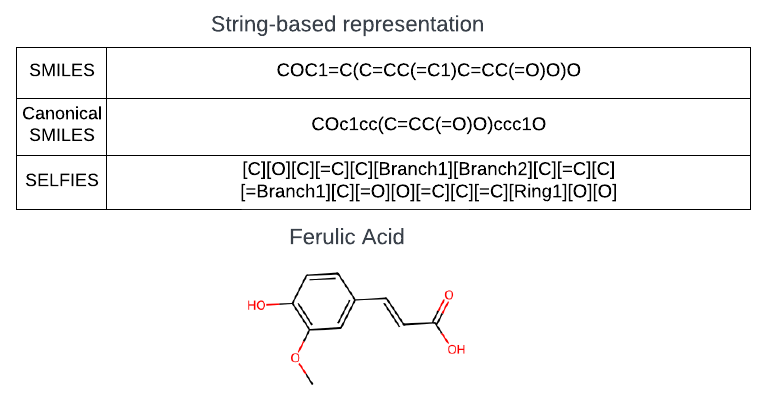
\includegraphics[scale=1]{3.png}
  \caption{String Based Representations of Ferulic Acid  }
  \label{fig:myfig}
\end{figure}


Deep learning model solution in chemistry domain is depended on how the molecular data is represented. The Simplified Molecular Input Line Entry System (SMILES) is a “chemical language” \cite{weiningerSMILESChemicalLanguage1988} that encodes structural information of a chemical into a compact text representation.. By mapping atoms to characters and bonds to punctuation, SMILES transforms the molecule structure of a molecule into a linear sequence. For example, c and C denote aromatic and aliphatic carbons respectively. Special characters like ‘=’ denote the type of bonds (connections between atoms). Rings are denoted by encapsulating numbers, and side chains by round brackets. 

The main advantage of the SMILES representation is its compatibility deep learning architectures developed for Natural Language Processing (NLP). By treating molecules as text, we can directly leverage sequence processing models such as Recurrent Neural Networks (RNNs), Long Short-Term Memory (LSTM) networks, and Transformers to train the Deep learning models.
therefore datasets with SMILES representation of molecules was used this project as it aligns with our objective of developing computationally efficient property prediction models

Therefore, datasets with SMILES representation of molecules were used in this project, as it aligns with our objective of developing computationally efficient property prediction models.

\begin{figure}[H]
  \centering
  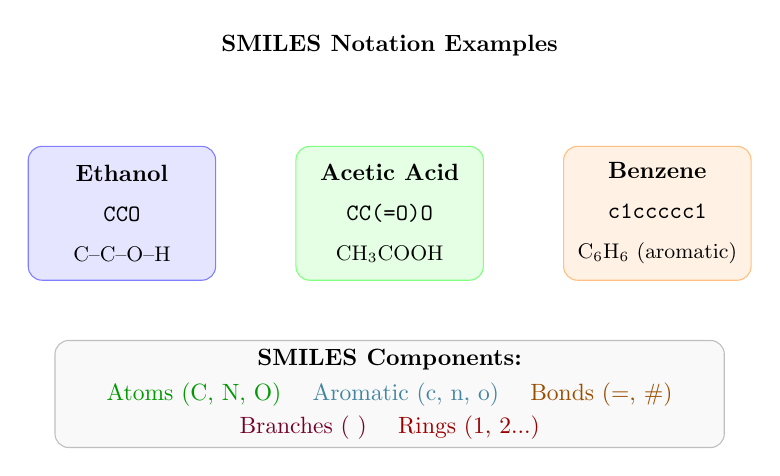
\begin{tikzpicture}[scale=0.85, transform shape]
    
    % Title
    \node[font=\bfseries] at (0, 4) {SMILES Notation Examples};
    
    % Example 1: Ethanol
    \begin{scope}[shift={(-4, 1.5)}]
      \node[draw=blue!50, rounded corners=5pt, fill=blue!10, 
            minimum width=2.8cm, minimum height=2cm, align=center] {
        \textbf{Ethanol}\\[5pt]
        \texttt{CCO}\\[5pt]
        \small C--C--O--H
      };
    \end{scope}
    
    % Example 2: Acetic Acid
    \begin{scope}[shift={(0, 1.5)}]
      \node[draw=green!50, rounded corners=5pt, fill=green!10, 
            minimum width=2.8cm, minimum height=2cm, align=center] {
        \textbf{Acetic Acid}\\[5pt]
        \texttt{CC(=O)O}\\[5pt]
        \small CH$_3$COOH
      };
    \end{scope}
    
    % Example 3: Benzene
    \begin{scope}[shift={(4, 1.5)}]
      \node[draw=orange!50, rounded corners=5pt, fill=orange!10, 
            minimum width=2.8cm, minimum height=2cm, align=center] {
        \textbf{Benzene}\\[5pt]
        \texttt{c1ccccc1}\\[5pt]
        \small C$_6$H$_6$ (aromatic)
      };
    \end{scope}
    
    % Legend - two rows
    \node[draw=gray!50, rounded corners=5pt, fill=gray!5, 
          minimum width=10cm, minimum height=1.6cm, align=center] at (0, -1.2) {
      \textbf{SMILES Components:}\\[3pt]
      \textcolor{green!60!black}{Atoms (C, N, O)} \quad
      \textcolor{cyan!60!black}{Aromatic (c, n, o)} \quad
      \textcolor{orange!60!black}{Bonds (=, \#)}\\[2pt]
      \textcolor{purple!60!black}{Branches ( )} \quad
      \textcolor{red!60!black}{Rings (1, 2...)}
    };
    
  \end{tikzpicture}
  \caption{Examples of SMILES notation for common molecules. SMILES encodes molecular structures as linear strings using specific symbols for atoms, bonds, branches, and ring closures.}
  \label{fig:smiles_examples}
\end{figure}

\subsection{Data Quality And Quantity}

The practical applicability and performance of any data-driven model are highly dependent on the degree of data quality and domain specificity in the chemistry domain. This is especially true in the domain of UV absorbing molecules, where the single greatest challenge in developing data driven solutions for property prediction and generative tasks is the lack of domain specific training data.

Therefore, it is essential to implement a data engineering strategy to develop and assemble databases relevant to UV-absorbing molecules.

Building and assembling domain-specific datasets is essential in our approach to developing UV-absorbing biobased compounds using novel computational approaches. 



Therefore, the lack of domain-specific datasets was addressed. Domain-specific datasets were developed that align with features as mentioned in Figure 1.2\textcolor{ForestGreen} {(a)}, such as, but not limited to, UV-Vis absorption maxima $\lambda_{max}$, Molecular Weight, The Topological Polar Surface Area (TPSA), Toxicity, Solubility, Octanol-Water partition coefficient (logP), SAS: Synthetic Accessibility Score, Natural product-likeness score (NP Score), Molar Extinction Coefficient, HOMO-LUMO Gap and Toxicity.
% Our expertise and access to experimental procedures largely eliminate the technical risk involved in having access to high-quality, diverse, and sufficient training data.
% \cite{Designing_mols}

Many publicly available datasets related to the above-mentioned properties have not been studied or integrated into a deep learning generative framework. Therefore, this project explored unexplored, high-quality, publicly available datasets related to these properties. 




Some of the dataset information and their unique challenges are discussed below. Some datasets are open-sourced, and some datasets can be purchased. 


 \textbf{UV-Vis absorption maximum - $\lambda_{max}$} 
 
UV-Vis absorption maximum - $\lambda_{max}$ of a specific molecule refers to the peak absorption wavelength in the UV-Vis absorption spectrum of that molecule. It provides information about the electronic structure of molecules, and it is a vital property in analyzing the UV-absorbing properties. 
% \begin{wrapfigure}{r}{0.5\textwidth} % 'r' for right, 'l' for left
%     \centering
%     
\includegraphics[width=0.5\textwidth]{sections/pics/UV.jpg} % replace 'your-image.jpg' with the image file name
%     \caption{UV-Vis Spectrum}
% \end{wrapfigure}

% This is an example text that will wrap around the image. You can add as much text as you want here, and it will continue to flow around the image, as long as there is enough space on the page. 

% You can add more content here to see the wrapping effect. Adjust the width of the wrapfigure environment to control how much space the image takes up.

Chromophores (carbonyl, nitro, azo, and other functional groups) are responsible for UV-Vis absorption. The presence and structure of these groups heavily influence $\lambda_{max}$ \cite{koplikUltravioletVisibleSpectrometry}, \cite{clarkWhatCausesMolecules2013}. The experimental database of optical properties of organic compounds \cite{joungExperimentalDatabaseOptical2020} is a database on the optical properties of organic chromophores. This dataset contains 20,236 data points and 7,016 unique organic chromophores in 365 solvents or in the solid state, which was developed by collecting the optical properties of organic compounds already reported in the literature.
Comparative dataset of experimental and computational attributes of UV-Vis absorption spectra \cite{beardComparativeDatasetExperimental2019} contains an auto generated database of 18,309 records of experimentally determined UV-vis
absorption maxima and associated extinction coefficients where present.

% The total dataset of
% 8,488 unique compounds and a subset of 5,380 compounds with experimental and computational
% data, are available in MongoDB, CSV and JSON formats. These can be queried using Python,
% R, Java, and MATLAB, for data-driven optoelectronic materials discovery.

One of the main challenges in integrating UV-Vis absorption maximum - $\lambda_{max}$ information into the deep learning solution is that UV-Vis absorption maximum - $\lambda_{max}$ is \textbf{measured with respect to a solvent}. Therefore, the corresponding solvent information and its \textbf{respective molecule information should be considered together}. \textbf{These solvents are not uniform across datasets or even within the same dataset}, as seen in the above databases.

 \textbf{HOMO-LUMO gap }(Highest Occupied Molecular Orbital - Lowest Unoccupied Molecular Orbital) 
 
 HOMO-LUMO gap is a quantum chemical property that refers to the energy difference between the highest energy level that electrons occupy (HOMO) and the lowest energy level that is unoccupied but can be accessed by electrons (LUMO). The HOMO-LUMO gap directly relates to the wavelength of light a molecule can absorb \cite{flemingMolecularOrbitalsOrganic2009}. Therefore, integrating HOMO-LUMO gap data into the solution framework is important for creating novel, optimized UV-absorbing molecules.
\cite{blanchardAISDHOMOLUMO2022} presents 1,048,576 molecules with HOMO-LUMO gap calculated using DFTB. \cite{lupopasiniTwoExcitedstateDatasets2023} presents two open-source datasets relating to organic molecules' HOMO-LUMO property. Each dataset contains 96,766 and 10,502,904 molecules of data, respectively. 

\textbf{Octanol-Water partition coefficient (logP)} 

Octanol-Water partition coefficient (logP) is a critical parameter in evaluating the drug-likeness of a molecule. Molecules with extreme logP values tend to have poor solubility and absorption, affecting their bioavailability\cite{atanasovNaturalProductsDrug2021}\cite{lipinskiExperimentalComputationalApproaches2001}. logP is integral to assessing ADMET (absorption, distribution, metabolism, excretion, and toxicity) profiles. Molecules with logP values that are too high may have increased toxicity, while those with low logP may suffer from poor permeability\cite{vandewaterbeemdADMETSilicoModelling2003}. During de novo molecule generation, controlling logP values helps generate molecules that are more likely to have favorable pharmacokinetics.\cite{martelLargeChemicallyDiverse2013} is an experimental data collection of 707 validated logP values for the development of new approaches to predict octanol/water partition coefficients of chemical compounds. And also RDKit’s rdkit.Chem.Crippen\cite{wildmanPredictionPhysicochemicalParameters1999} module can be used to calculate logP values from SMILES representation.

\textbf{SAS: Synthetic Accessibility Score} 

SAS: The Synthetic Accessibility Score is a metric used in cheminformatics and drug discovery to estimate the ease with which a given molecular structure can be synthesized in a laboratory setting, which is an important consideration. A low SAS value indicates a relatively easy molecule to synthesize, while a high SAS value suggests a more complex and potentially challenging synthesis. SAS is particularly useful in de novo molecule generation to help prioritize compounds based on their synthetic feasibility. RDKit-based estimation or score based on the molecule symmetry method\cite{ertlEstimationSyntheticAccessibility2009} can be used for this calculation.

\textbf{Natural product-likeness score (NP Score)} 

Through the evolutionary selection process, natural products often contain bioactive substructures that can be utilized in UV compounds\cite{atanasovNaturalProductsDrug2021}. The NP score for a molecule quantifies how similar its substructure is to that of natural products. A higher score indicates that the molecular structure is more likely within the natural product space\cite{ertlNaturalProductlikenessScore2008}.

\subsection{Data Engineering}

There are certain challenges in using these chemical datasets. Most of the above-mentioned
datasets are not uniform. They come from different parts of the chemical space. They are often
incomplete with missing data points. They offer different molecular representations. Therefore,
considerable data engineering effort was carried out to filter, process, clean, and transform
these into forms suitable for model training and inference. As described below, string-based
representation was used as a molecular representation, and data engineering
was carried out to transform the data sets into a uniform structure that is useful for model
training.



\subsection{UV absorption max }

As it was identified that the UV absorption property of small molecules is helpful industrial
applications, Deep Learning models based on RNN models were developed
to predict the UV absorption maximum given a chemical molecule. This enables us to predict the wavelength at which a particular molecule absorbs the most UV energy.

\begin{figure}[H]
  \centering
  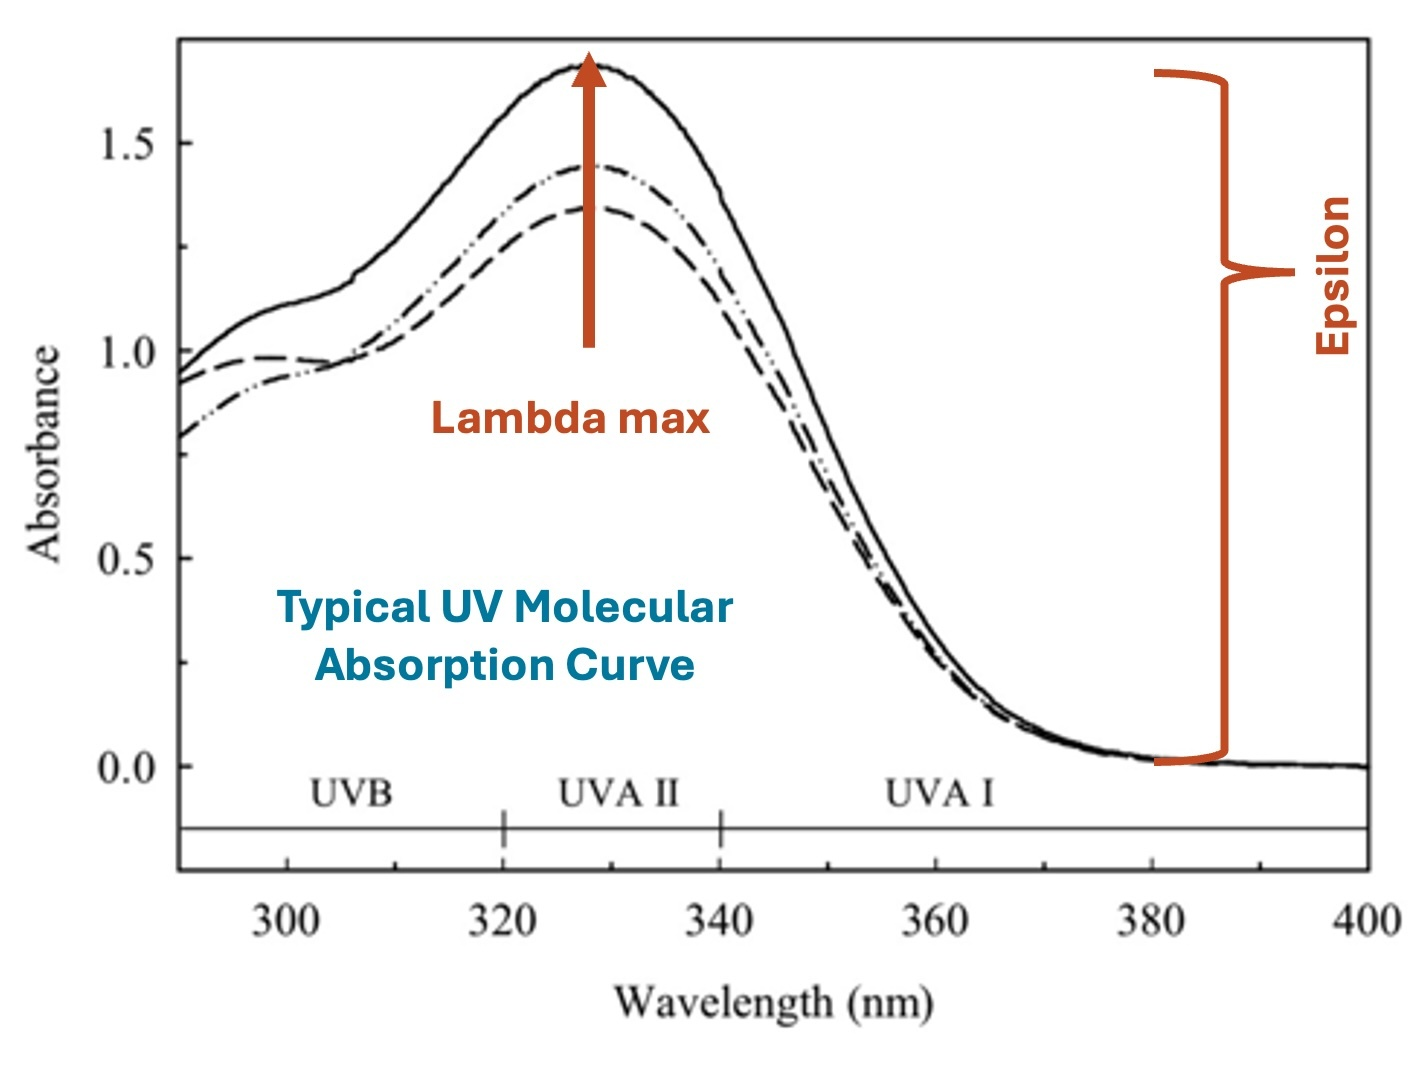
\includegraphics[scale=0.2]{UV.jpg}
  \caption{UV Molecular Absorption Curve  }
  \label{fig:myfig}
\end{figure}

Our primary focus was prediction of the maximum absorption wavelength ($\lambda_{max}$). This property is the useful and important  metric for analyzing the electronic structure and function of UV-absorbing molecules. This property dictates a molecule's suitability for applications in this domain \cite{giokasUVFiltersSunscreens2007}\cite{jesusUVFiltersChallenges2022a}.



\section{Related Work}


The Simplified Molecular-Input Line-Entry System (SMILES) provides a text-based representation of molecules that enables the application of natural language processing (NLP) techniques to chemical structures \citep{weiningerSMILESChemicalLanguage1988}. As SMILES strings are sequential and composed of characters, methods inspired by NLP such as word embeddings and recurrent neural networks have been extensively explored for molecular property prediction \citep{gohSMILES2VecInterpretableGeneralPurpose2018}.

Early deep learning approaches for SMILES-based property prediction employed recurrent neural networks (RNNs). \citet{xuSeq2seqFingerprintUnsupervised2017} introduced Seq2seq fingerprint, which learns molecular embeddings using encoder-decoder RNN architectures in an unsupervised manner. Long Short-Term Memory (LSTM) and Gated Recurrent Unit (GRU) networks have gained widespread adoption for processing SMILES sequences due to their ability to capture long-range dependencies \citep{GeneratingFocusedMolecule}. \citet{gohSMILES2VecInterpretableGeneralPurpose2018} proposed SMILES2vec, an interpretable deep neural network that processes SMILES strings for predicting chemical properties. Bidirectional LSTM architectures have shown particular promise, demonstrating that BiLSTM models with attention mechanisms achieve competitive performance in predicting aqueous solubility and partition coefficients.

Convolutional neural networks (CNNs) have also been applied to SMILES-based prediction. \citet{hiroharaConvolutionalNeuralNetwork2018a} proposed SCFP (SMILES-based Convolutional Fingerprint), which processes one-hot encoded SMILES vectors using convolutional layers. 

The introduction of Transformer architectures has significantly advanced molecular property prediction. \citet{wangSMILESBERTLargeScale2019} developed SMILES-BERT, adapting the BERT framework for molecular representations through masked token prediction on large-scale unlabeled SMILES data. \citet{honda2019smiles} proposed SMILES Transformer for pre-trained molecular fingerprints, demonstrating effectiveness in low-data drug discovery scenarios. 

Recognizing that different molecular representations capture complementary information, hybrid approaches have emerged. GraSeq \citep{guoGraSeqGraphSequence2020} combines SMILES sequences with molecular graphs using LSTM and graph neural networks to capture both sequential and topological information. MTBG \citep{liuPredictionMolecularToxicity2023} integrates SMILES processing via BiGRU with molecular graph embeddings using GraphSAGE for toxicity prediction.

\subsection{Comparative Studies: RNN vs Transformer}

\citet{chenMolecularLanguageModels2023} conducted a systematic comparison of RNN-based and Transformer-based language models across three molecular generation tasks of varying complexity. Their findings revealed that the optimal architecture choice depends on the characteristics of the target property. Specifically, RNNs demonstrated superior performance on tasks where molecular properties are determined by local structural features, while Transformers excelled when global molecular architecture and long-range dependencies were paramount.

Several factors support the selection of RNNs for UV absorption prediction:

\textbf{Local Feature Dependence.} UV-Vis absorption maxima ($\lambda_{max}$) are primarily governed by chromophoric groups and their immediate electronic environments. The $\pi \rightarrow \pi^*$ and $n \rightarrow \pi^*$ transitions responsible for UV absorption arise from localized conjugated systems, carbonyl groups, and aromatic rings. \citet{chenMolecularLanguageModels2023} demonstrated that RNNs outperform Transformers on properties such as logP, which are computed as sums of atomic contributions, a paradigm analogous to how electronic transitions depend on local chromophore contributions. The partition coefficient logP shares computational similarities with UV absorption, as both properties can be decomposed into contributions from molecular substructures.

\textbf{Moderate Sequence Lengths.} The molecules in our dataset, comprising sunscreen compounds and phenolic acids, exhibit moderate molecular weights and SMILES sequence lengths typically ranging from 30 to 80 tokens. \citet{chenMolecularLanguageModels2023} found that RNNs perform optimally in this regime, with performance degradation occurring primarily for large molecules exceeding 100 heavy atoms. The Transformer's advantage in capturing long-range dependencies becomes relevant only for sequences substantially longer than those in our dataset.

\textbf{Sequential Structure Encoding.} SMILES strings encode molecular structure in a manner where adjacent tokens often represent chemically connected atoms. RNNs naturally capture these local adjacency relationships through their recurrent hidden state updates. For chromophore identification, the sequential processing of RNNs aligns well with tracing conjugation pathways through the molecular graph as encoded in the SMILES representation.

\textbf{Computational Efficiency.} For our dataset size and sequence lengths, RNNs offer favorable computational characteristics. The quadratic attention complexity of Transformers with respect to sequence length provides no advantage for moderate-length SMILES strings, while RNNs achieve comparable or superior performance with linear complexity.

It should be noted that Transformers may offer advantages for related tasks involving larger molecules or properties requiring global structural awareness. However, for the specific application of predicting UV absorption wavelengths in small to medium-sized organic chromophores, the empirical evidence and theoretical considerations favor RNN-based architectures.


\section{Methods}

\subsection{Dataset Description and Preparation}


The accurate prediction of UV absorption properties for small molecules has significant implications for industrial applications, including pharmaceutical development, sunscreen formulation, and optoelectronic materials design. To build a robust machine learning model capable of predicting UV absorption maxima ($\lambda_{max}$) for organic compounds, we identified and combined two comprehensive experimental databases from the literature. The selection criteria prioritized datasets with: (1) experimentally validated absorption measurements, (2) standardized SMILES representations for molecular structures, (3) documented solvent information, and (4) sufficient size and chemical diversity for training deep learning models.

\subsection{Dataset 1: Experimental Database of Optical Properties of Organic Compounds}

The first dataset employed in this study is the Experimental Database of Optical Properties of Organic Compounds, developed by Joung et al. \cite{joungExperimentalDatabaseOptical2020}. This database was specifically curated to facilitate data-driven chemistry applications using machine learning approaches. The dataset was constructed by systematically collecting optical properties of organic compounds from previously published literature sources.

The database comprises 20,236 data points spanning 7,016 unique organic chromophores measured in 365 different solvents or in the solid state. The optical properties recorded are derived from absorption and emission spectra as reported in the original publications. Table~\ref{tab:dataset1_format} describes the data fields available in this database.

\begin{table}[H]
\centering
\caption{Data fields in the Experimental Database of Optical Properties of Organic Compounds.}
\label{tab:dataset1_format}
\begin{tabular}{ll}
\toprule
\textbf{Field} & \textbf{Description} \\
\midrule
SMILES & Canonical SMILES representation of the molecule \\
Solvent & Solvent used for measurement \\
Absorption max (nm) & Wavelength of maximum absorption \\
Emission max (nm) & Wavelength of maximum emission \\
Quantum yield & Fluorescence quantum yield \\
Extinction coefficient & Molar extinction coefficient \\
Reference & Original literature source \\
\bottomrule
\end{tabular}
\end{table}

The comprehensive coverage of solvent conditions in this dataset makes it particularly valuable for our solvent-aware prediction approach, as it enables the model to learn solvatochromic effects across a diverse range of solute-solvent combinations.

\subsection{Dataset 2: Comparative Dataset of UV/Vis Absorption Spectra}

The second dataset utilized is the Comparative Dataset of Experimental and Computational Attributes of UV/Vis Absorption Spectra, developed by Beard et al. \cite{beardComparativeDatasetExperimental2019}. This database was auto-generated through systematic extraction from the literature and contains 18,309 records of experimentally determined UV/Vis absorption maxima along with associated extinction coefficients where available.

The dataset encompasses 8,488 unique compounds, with a subset of 5,380 compounds containing both experimental and computational data. The database is provided in multiple formats including MongoDB, CSV, and JSON, facilitating integration with various programming environments such as Python, R, Java, and MATLAB.
\begin{table}[H]
\centering
\caption{Summary of Dataset 2 characteristics.}
\label{tab:dataset2_summary}
\begin{tabular}{ll}
\toprule
\textbf{Attribute} & \textbf{Value} \\
\midrule
Total records & 18,309 \\
Unique compounds & 8,488 \\
Compounds with experimental + computational data & 5,380 \\
Available formats & MongoDB, CSV, JSON \\
Primary properties & $\lambda_{max}$, extinction coefficient \\
\bottomrule
\end{tabular}
\end{table}

To maximize the training data available for our deep learning model, we combined both datasets.

\subsection{Neural Network Architecture}

Recurrent Neural Networks (RNNs) are designed to process sequential data by maintaining a hidden state that captures information from previous time steps. One of the main challenges in applying RNN networks is designing an appropriate network architecture. The optimal combination of various network parameters (types and sizes of network layers, activation and optimization functions, learning and dropout rates, and the optimal way to encode the training data into vectorized form required by the network) requires some trial and error. There are no general rules for designing the optimal architecture; one has to experiment with different architectures and parameters.

This section presents our best performing complete model architecture ( and others we tried as well) for SMILES-based molecular property prediction. The model integrates embedding, bidirectional GRU layers, and fully connected layers.

To use SMILES strings as input to neural networks, they must be converted to numerical representations through the following steps:

\begin{enumerate}
    \item \textbf{Tokenization}: Split the SMILES string into individual tokens (characters or multi-character symbols like \texttt{Cl}, \texttt{Br}).
    \item \textbf{Vocabulary Mapping}: Map each unique token to an integer index.
    \item \textbf{Padding}: Pad sequences to a fixed maximum length $T_{\max}$ for batch processing.
    \item \textbf{Embedding}: Convert integer indices to dense vector representations.
\end{enumerate}

\begin{figure}[H]
  \centering
  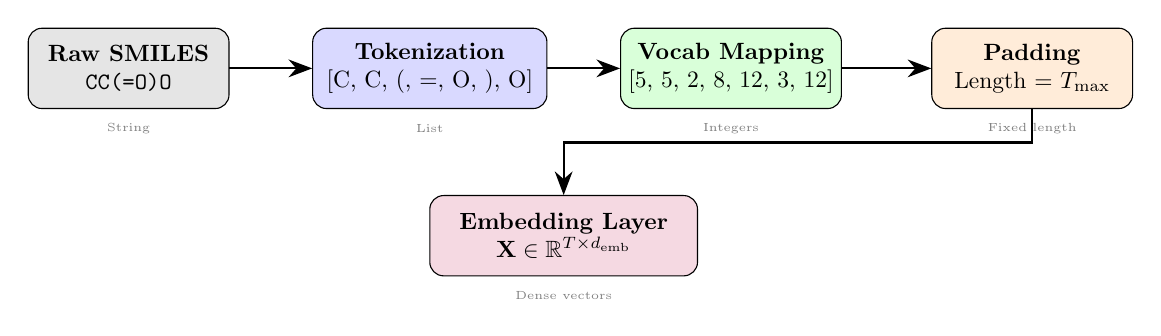
\begin{tikzpicture}[scale=0.85, transform shape,
    box/.style={draw, rounded corners=5pt, minimum height=1.2cm, align=center},
    arrow/.style={-{Stealth[length=3mm]}, thick}
  ]
    
    % Stage 1: Raw SMILES
    \node[box, fill=gray!20, minimum width=3cm] (raw) at (-6, 0) {
      \textbf{Raw SMILES}\\
      \texttt{CC(=O)O}
    };
    
    % Stage 2: Tokenization
    \node[box, fill=blue!15, minimum width=3.5cm] (token) at (-1.5, 0) {
      \textbf{Tokenization}\\
      {[C, C, (, =, O, ), O]}
    };
    
    % Stage 3: Vocabulary Mapping
    \node[box, fill=green!15, minimum width=3cm] (vocab) at (3, 0) {
      \textbf{Vocab Mapping}\\
      {[5, 5, 2, 8, 12, 3, 12]}
    };
    
    % Stage 4: Padding
    \node[box, fill=orange!15, minimum width=3cm] (pad) at (7.5, 0) {
      \textbf{Padding}\\
      Length = $T_{\max}$
    };
    
    % Stage 5: Embedding (below)
    \node[box, fill=purple!15, minimum width=4cm] (embed) at (0.5, -2.5) {
      \textbf{Embedding Layer}\\
      $\mathbf{X} \in \mathbb{R}^{T \times d_{\text{emb}}}$
    };
    
    % Arrows
    \draw[arrow] (raw) -- (token);
    \draw[arrow] (token) -- (vocab);
    \draw[arrow] (vocab) -- (pad);
    \draw[arrow] (pad.south) -- ++(0, -0.5) -| (embed.north);
    
    % Dimension annotations
    \node[font=\tiny, gray] at (-6, -0.9) {String};
    \node[font=\tiny, gray] at (-1.5, -0.9) {List};
    \node[font=\tiny, gray] at (3, -0.9) {Integers};
    \node[font=\tiny, gray] at (7.5, -0.9) {Fixed length};
    \node[font=\tiny, gray] at (0.5, -3.4) {Dense vectors};
    
  \end{tikzpicture}
  \caption{SMILES processing pipeline for neural network input. Raw SMILES strings are tokenized, mapped to integers via a vocabulary, padded to fixed length, and embedded into dense vector representations.}
  \label{fig:smiles_pipeline}
\end{figure}

\tikzstyle{startstop} = [rectangle, rounded corners, minimum width=3cm, minimum height=1cm,text centered, draw=black]
\tikzstyle{process} = [rectangle, minimum width=3cm, minimum height=1cm, text centered, draw=black]
\tikzstyle{arrow} = [thick,->,>=stealth]


The model consists of the following components:

\begin{enumerate}
    \item \textbf{Embedding Layer}: Maps tokenized SMILES characters to dense vectors of dimension 50.
    
    \item \textbf{Bidirectional GRU Layer 1}: Processes embedded sequences bidirectionally with 128 hidden units per direction, outputting 128-dimensional hidden states.
    
    \item \textbf{Bidirectional GRU Layer 2}: Further processes the sequence with another BiGRU layer (128 units per direction), capturing higher-level sequential patterns.
    
    \item \textbf{Global Average Pooling}: Aggregates variable-length sequences into fixed-length vectors by averaging across time steps.
    
    \item \textbf{Dense Layer}: A fully connected layer with 128 units and ReLU activation transforms the pooled representation.
    
    \item \textbf{Dropout Layer}: Applies dropout with rate 0.2 for regularization.
    
    \item \textbf{Output Layer}: A linear layer produces the final property prediction.
\end{enumerate}

% ============================================================================
% FIGURE: Complete Model Architecture
% ============================================================================
\begin{figure}[H]
  \centering
  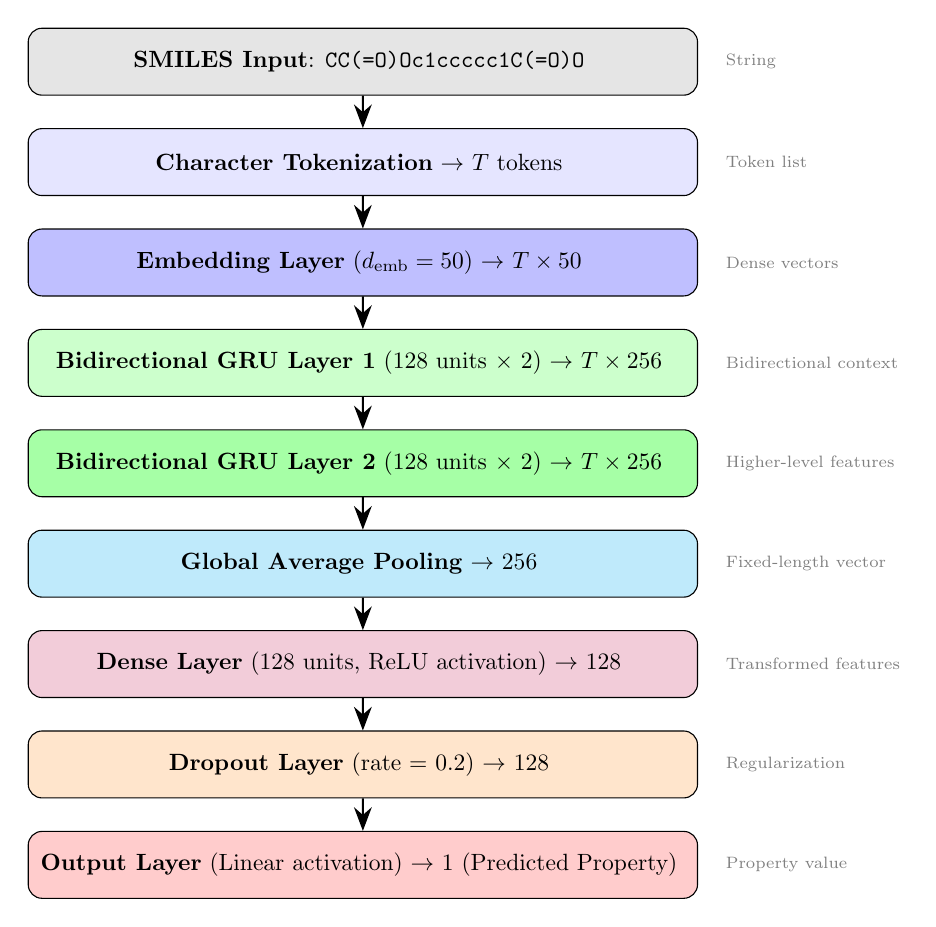
\begin{tikzpicture}[scale=0.85, transform shape,
    layer/.style={draw, rounded corners=5pt, minimum width=10cm, minimum height=1cm, align=center},
    arrow/.style={-{Stealth[length=3mm]}, thick}
  ]
    
    % Input
    \node[layer, fill=gray!20] (input) at (0, 0) {
      \textbf{SMILES Input}: \texttt{CC(=O)Oc1ccccc1C(=O)O}
    };
    
    % Tokenization
    \node[layer, fill=blue!10] (token) at (0, -1.5) {
      \textbf{Character Tokenization} $\rightarrow$ $T$ tokens
    };
    
    % Embedding
    \node[layer, fill=blue!25] (embed) at (0, -3) {
      \textbf{Embedding Layer} ($d_{\text{emb}} = 50$) $\rightarrow$ $T \times 50$
    };
    
    % BiGRU 1
    \node[layer, fill=green!20] (bigru1) at (0, -4.5) {
      \textbf{Bidirectional GRU Layer 1} (128 units $\times$ 2) $\rightarrow$ $T \times 256$
    };
    
    % BiGRU 2
    \node[layer, fill=green!35] (bigru2) at (0, -6) {
      \textbf{Bidirectional GRU Layer 2} (128 units $\times$ 2) $\rightarrow$ $T \times 256$
    };
    
    % Global Pooling
    \node[layer, fill=cyan!25] (pool) at (0, -7.5) {
      \textbf{Global Average Pooling} $\rightarrow$ 256
    };
    
    % Dense
    \node[layer, fill=purple!20] (dense) at (0, -9) {
      \textbf{Dense Layer} (128 units, ReLU activation) $\rightarrow$ 128
    };
    
    % Dropout
    \node[layer, fill=orange!20] (dropout) at (0, -10.5) {
      \textbf{Dropout Layer} (rate = 0.2) $\rightarrow$ 128
    };
    
    % Output
    \node[layer, fill=red!20] (output) at (0, -12) {
      \textbf{Output Layer} (Linear activation) $\rightarrow$ 1 (Predicted Property)
    };
    
    % Arrows
    \draw[arrow] (input) -- (token);
    \draw[arrow] (token) -- (embed);
    \draw[arrow] (embed) -- (bigru1);
    \draw[arrow] (bigru1) -- (bigru2);
    \draw[arrow] (bigru2) -- (pool);
    \draw[arrow] (pool) -- (dense);
    \draw[arrow] (dense) -- (dropout);
    \draw[arrow] (dropout) -- (output);
    
    % Dimension annotations (right side)
    \node[font=\scriptsize, gray, right] at (5.3, 0) {String};
    \node[font=\scriptsize, gray, right] at (5.3, -1.5) {Token list};
    \node[font=\scriptsize, gray, right] at (5.3, -3) {Dense vectors};
    \node[font=\scriptsize, gray, right] at (5.3, -4.5) {Bidirectional context};
    \node[font=\scriptsize, gray, right] at (5.3, -6) {Higher-level features};
    \node[font=\scriptsize, gray, right] at (5.3, -7.5) {Fixed-length vector};
    \node[font=\scriptsize, gray, right] at (5.3, -9) {Transformed features};
    \node[font=\scriptsize, gray, right] at (5.3, -10.5) {Regularization};
    \node[font=\scriptsize, gray, right] at (5.3, -12) {Property value};
    
  \end{tikzpicture}
  \caption{Complete model architecture for SMILES-based molecular property prediction. The model processes SMILES strings through embedding, stacked bidirectional GRU layers, global average pooling, and fully connected layers with dropout regularization.}
  \label{fig:complete_architecture}
\end{figure}

% % ============================================================================
% % FIGURE: Complete Model Architecture with Description (Side by Side)
% % ============================================================================
% \begin{figure}[H]
%   \centering
%   \begin{minipage}[c]{0.38\textwidth}
%     \small
%     \textbf{Layer Descriptions:}
%     \begin{enumerate}[leftmargin=*, itemsep=2pt, parsep=0pt]
%       \item \textbf{Embedding}: Maps tokens to dense vectors (dim=50)
%       \item \textbf{BiGRU Layer 1}: 128 units $\times$ 2 directions
%       \item \textbf{BiGRU Layer 2}: 128 units $\times$ 2 directions
%       \item \textbf{Global Avg Pooling}: Aggregates to fixed-length
%       \item \textbf{Dense Layer}: 128 units, ReLU activation
%       \item \textbf{Dropout}: Rate = 0.2
%       \item \textbf{Output}: Linear activation $\rightarrow$ 1
%     \end{enumerate}
%   \end{minipage}
%   \hfill
%   \begin{minipage}[c]{0.58\textwidth}
%     \centering
%     \begin{tikzpicture}[scale=0.65, transform shape,
%       layer/.style={draw, rounded corners=4pt, minimum width=7cm, minimum height=0.7cm, align=center, font=\small},
%       arrow/.style={-{Stealth[length=2mm]}, thick}
%     ]
      
%       \node[layer, fill=gray!20] (input) at (0, 0) {
%         \textbf{SMILES}: \texttt{CC(=O)Oc1ccccc1C(=O)O}
%       };
      
%       \node[layer, fill=blue!10] (token) at (0, -1.1) {
%         \textbf{Tokenization} $\rightarrow$ $T$ tokens
%       };
      
%       \node[layer, fill=blue!25] (embed) at (0, -2.2) {
%         \textbf{Embedding} ($d=50$) $\rightarrow$ $T \times 50$
%       };
      
%       \node[layer, fill=green!20] (bigru1) at (0, -3.3) {
%         \textbf{BiGRU-1} (128$\times$2) $\rightarrow$ $T \times 256$
%       };
      
%       \node[layer, fill=green!35] (bigru2) at (0, -4.4) {
%         \textbf{BiGRU-2} (128$\times$2) $\rightarrow$ $T \times 256$
%       };
      
%       \node[layer, fill=cyan!25] (pool) at (0, -5.5) {
%         \textbf{Global Avg Pool} $\rightarrow$ 256
%       };
      
%       \node[layer, fill=purple!20] (dense) at (0, -6.6) {
%         \textbf{Dense} (128, ReLU) $\rightarrow$ 128
%       };
      
%       \node[layer, fill=orange!20] (dropout) at (0, -7.7) {
%         \textbf{Dropout} (0.2) $\rightarrow$ 128
%       };
      
%       \node[layer, fill=red!20] (output) at (0, -8.8) {
%         \textbf{Output} (Linear) $\rightarrow$ 1
%       };
      
%       \draw[arrow] (input) -- (token);
%       \draw[arrow] (token) -- (embed);
%       \draw[arrow] (embed) -- (bigru1);
%       \draw[arrow] (bigru1) -- (bigru2);
%       \draw[arrow] (bigru2) -- (pool);
%       \draw[arrow] (pool) -- (dense);
%       \draw[arrow] (dense) -- (dropout);
%       \draw[arrow] (dropout) -- (output);
      
%     \end{tikzpicture}
%   \end{minipage}
%   \caption{Complete model architecture for SMILES-based molecular property prediction. The model processes SMILES strings through embedding, stacked bidirectional GRU layers, global average pooling, and fully connected layers with dropout regularization.}
%   \label{fig:complete_architecture}
% \end{figure}



% \begin{figure}[ht]
% \centering


% \begin{tikzpicture}[node distance=2cm]
% \node (start) [startstop] {Dense Layer - 1000};
% \node (pro1) [process, below of=start] {Dropout layer - 0.20};
% \node (pro2) [process, below of=pro1] {Dense Layer - 1000};



% \draw [arrow] (start) -- (pro1);
% \draw [arrow] (pro1) -- (pro2);



% \end{tikzpicture}

% \caption{ Encoder and Decoder Architecture }


% \end{figure}
% \newpage
% \newpage


\tikzstyle{startstop} = [rectangle, rounded corners, minimum width=3cm, minimum height=1cm, text centered, draw=black]
\tikzstyle{process} = [rectangle, minimum width=3cm, minimum height=1cm, text centered, draw=black]
\tikzstyle{arrow} = [thick,->,>=stealth]

\begin{figure}[H]
\centering

% Top row - two figures side by side
\begin{minipage}[t]{0.48\textwidth}
\centering
\begin{tikzpicture}[node distance=1.5cm, scale=0.85, transform shape]
\node (start) [startstop] {Embedding Layer - 50};
\node (pro1) [process, below of=start] {Bidirectional GRU Layer - 128};
\node (pro2) [process, below of=pro1] {Bidirectional GRU Layer - 128};
\node (pro3) [process, below of=pro2] {Dense Layer (ReLU) - 128};
\node (pro4) [process, below of=pro3] {Dropout Layer - 0.2};
\node (pro5) [process, below of=pro4] {Dense Layer (Linear) - 128};
\draw [arrow] (start) -- (pro1);
\draw [arrow] (pro1) -- (pro2);
\draw [arrow] (pro2) -- (pro3);
\draw [arrow] (pro3) -- (pro4);
\draw [arrow] (pro4) -- (pro5);
\end{tikzpicture}
\subcaption{BiGRU Architecture}
\label{fig:bigru}
\end{minipage}
\hfill
\begin{minipage}[t]{0.48\textwidth}
\centering
\begin{tikzpicture}[node distance=1.5cm, scale=0.85, transform shape]
\node (start) [startstop] {Embedding Layer - 50};
\node (pro1) [process, below of=start] {Bidirectional LSTM Layer - 128};
\node (pro2) [process, below of=pro1] {Bidirectional LSTM Layer - 128};
\node (pro3) [process, below of=pro2] {Dense Layer (ReLU) - 128};
\node (pro4) [process, below of=pro3] {Dropout Layer - 0.2};
\node (pro5) [process, below of=pro4] {Dense Layer (Linear) - 128};
\draw [arrow] (start) -- (pro1);
\draw [arrow] (pro1) -- (pro2);
\draw [arrow] (pro2) -- (pro3);
\draw [arrow] (pro3) -- (pro4);
\draw [arrow] (pro4) -- (pro5);
\end{tikzpicture}
\subcaption{BiLSTM Architecture}
\label{fig:bilstm}
\end{minipage}

\vspace{1cm}

% Bottom row - one figure centered
\begin{minipage}[t]{0.5\textwidth}
\centering
\begin{tikzpicture}[node distance=1.5cm, scale=0.85, transform shape]
\node (start) [startstop] {Embedding Layer - 50};
\node (pro1) [process, below of=start] {Conv1D Layer - 192, 3};
\node (pro2) [process, below of=pro1] {Bidirectional GRU Layer - 128};
\node (pro3) [process, below of=pro2] {Bidirectional GRU Layer - 128};
\node (pro4) [process, below of=pro3] {Dense Layer (ReLU) - 128};
\node (pro5) [process, below of=pro4] {Dropout Layer - 0.2};
\node (pro6) [process, below of=pro5] {Dense Layer (Linear) - 128};
\draw [arrow] (start) -- (pro1);
\draw [arrow] (pro1) -- (pro2);
\draw [arrow] (pro2) -- (pro3);
\draw [arrow] (pro3) -- (pro4);
\draw [arrow] (pro4) -- (pro5);
\draw [arrow] (pro5) -- (pro6);
\end{tikzpicture}
\subcaption{CNN-BiGRU Architecture}
\label{fig:cnn-bigru}
\end{minipage}

\caption{Neural network architectures tested for SMILES-based regression predictions of UV absorption max: (a) Bidirectional GRU, (b) Bidirectional LSTM, and (c) CNN-Bidirectional GRU hybrid.}
\label{fig:architectures}
\end{figure}

% \subsection{additional}

% \section{Sequence-based deep learning models for UV absorption maximum prediction}
% \label{sec:seq_uv_models}

% In this work, we develop sequence-based deep learning models for predicting the UV--visible absorption maximum, $\lambda_{\max}$, of small organic UV absorbers from their SMILES representations. The UV absorption maximum is a key photophysical descriptor for applications such as sunscreens, UV-protective coatings, and UV-stabilizing additives, and is closely related to the underlying electronic structure and conjugation pattern of the chromophore. Conventional quantitative structure--property relationship (QSPR) models for $\lambda_{\max}$ rely on handcrafted descriptors (e.g., conjugation length, Hammett parameters, quantum-chemical features), which can be expensive to compute and may generalize poorly to new chemical scaffolds.

% By contrast, sequence-based neural models treat SMILES strings as one-dimensional molecular ``languages'' and learn task-specific representations directly from the raw sequence. In particular, we employ gated recurrent neural networks (GRUs/LSTMs) over SMILES sequences to encode molecular structure into a fixed-size vector, which is then used to regress $\lambda_{\max}$ in nanometers. This section describes the input representation, recurrent architectures, and model design choices adopted for UV absorption maximum prediction.

% \subsection{Sequence representation and notation}
% \label{subsec:notation}

% Let a molecule be represented by a SMILES string $s$, which we treat as a sequence of discrete tokens:
% \begin{equation}
%   s = (c_1, c_2, \dots, c_T), \quad c_t \in \mathcal{V},
% \end{equation}
% where $T \in \mathbb{N}$ is the sequence length, and $\mathcal{V}$ is a finite vocabulary of SMILES tokens. Each token $c_t$ is mapped to a numerical input vector $x_t \in \mathbb{R}^{d_{\mathrm{emb}}}$ via an embedding layer (Section~\ref{subsec:input_representation}), producing an embedded sequence
% \begin{equation}
%   (x_1, x_2, \dots, x_T), \quad x_t \in \mathbb{R}^{d_{\mathrm{emb}}}.
% \end{equation}

% A recurrent encoder then computes hidden states
% \begin{equation}
%   h_t = f_{\mathrm{RNN}}(x_t, h_{t-1}; \theta), \quad h_t \in \mathbb{R}^{d_h},
% \end{equation}
% where $d_h$ is the hidden dimension and $\theta$ denotes the trainable parameters of the recurrent cell. Depending on the architecture, we may also maintain a cell state $c_t \in \mathbb{R}^{d_h}$ (for LSTMs). For bidirectional encoders, we obtain forward and backward hidden states at each position $t$, denoted by $\overrightarrow{h}_t$ and $\overleftarrow{h}_t$, which are concatenated to form a context-aware token representation
% \begin{equation}
%   h_t = [\,\overrightarrow{h}_t; \overleftarrow{h}_t\,] \in \mathbb{R}^{2d_h}.
% \end{equation}

% The sequence of hidden states $(h_1, \dots, h_T)$ is subsequently aggregated into a fixed-size molecular representation $h_{\mathrm{mol}}$ by an attention-based pooling layer (Section~\ref{subsec:design_choices}), which is then passed to dense layers to predict $\lambda_{\max}$.

% \subsection{Input representation: SMILES tokenization, one-hot encoding, and embeddings}
% \label{subsec:input_representation}

% \paragraph{Tokenization.}
% We adopt \emph{character-level} tokenization for SMILES strings due to its simplicity and robustness. The vocabulary $\mathcal{V}$ contains all SMILES characters observed in the dataset (e.g., atom symbols such as \texttt{C}, \texttt{N}, \texttt{O}; bond symbols such as \texttt{=}, \texttt{\#}; branching symbols \texttt{(}, \texttt{)}; ring indices; and brackets), augmented with special tokens:
% \begin{itemize}
%   \item \verb|<bos>|: beginning-of-sequence marker,
%   \item \verb|<eos>|: end-of-sequence marker,
%   \item \verb|<pad>|: padding token for batched training,
%   \item \verb|<unk>|: unknown token (optional, for rare/unseen characters).
% \end{itemize}
% Character-level tokenization avoids the need for dataset-specific parsing rules and works seamlessly with randomized SMILES augmentation (Section~\ref{subsec:design_choices}). It also ensures that the same tokenization scheme can be applied consistently across different UV absorber datasets.

% \paragraph{One-hot encoding.}
% Each token $c_t \in \mathcal{V}$ is mapped to an integer index
% \begin{equation}
%   k_t = \text{index}(c_t) \in \{1, 2, \dots, |\mathcal{V}|\},
% \end{equation}
% and then to a one-hot vector $o_t \in \{0,1\}^{|\mathcal{V}|}$ defined by
% \begin{equation}
%   (o_t)_j =
%   \begin{cases}
%     1, & \text{if } j = k_t, \\
%     0, & \text{otherwise}.
%   \end{cases}
% \end{equation}
% One-hot vectors are high-dimensional, sparse, and do not encode any inherent similarity between tokens (all distinct tokens are equidistant in Euclidean space). Consequently, they serve only as an intermediate representation and are not fed directly into the recurrent layers.

% \paragraph{Embedding layer.}
% To obtain compact and trainable token features, we introduce a learnable embedding matrix
% \begin{equation}
%   E \in \mathbb{R}^{|\mathcal{V}| \times d_{\mathrm{emb}}},
% \end{equation}
% with embedding dimension fixed to $d_{\mathrm{emb}} = 50$ in all experiments. The embedded input at time step $t$ is given by
% \begin{equation}
%   x_t = E^{\top} o_t \in \mathbb{R}^{d_{\mathrm{emb}}} = \mathbb{R}^{50},
% \end{equation}
% which is equivalent in practice to selecting the row of $E$ corresponding to token $c_t$. The embedding layer thus implements a mapping
% \begin{equation}
%   \text{Embed} : \mathcal{V} \to \mathbb{R}^{50}, \quad c_t \mapsto x_t.
% \end{equation}
% The parameters of $E$ are initialized randomly and learned jointly with the recurrent encoder and prediction head via backpropagation. Over the course of training, the model discovers a task-specific geometry in embedding space: tokens that play similar roles in SMILES (e.g., common heavy atoms or paired structural delimiters) may acquire similar embeddings, while tokens with distinct functional roles are separated. After embedding, each SMILES string is represented as
% \begin{equation}
%   (x_1, x_2, \dots, x_T), \quad x_t \in \mathbb{R}^{50},
% \end{equation}
% which serves as the input to the recurrent encoder.

% \subsection{Recurrent architectures: RNN, LSTM, and GRU}
% \label{subsec:rnn_architectures}

% \paragraph{Vanilla RNN.}
% The Elman RNN defines the hidden state update as
% \begin{equation}
%   h_t = \phi\left( W_{xh} x_t + W_{hh} h_{t-1} + b_h \right),
% \end{equation}
% where $W_{xh} \in \mathbb{R}^{d_h \times d_{\mathrm{emb}}}$, $W_{hh} \in \mathbb{R}^{d_h \times d_h}$, $b_h \in \mathbb{R}^{d_h}$, and $\phi(\cdot)$ is a nonlinear activation (typically $\tanh$). Although conceptually simple, vanilla RNNs suffer from vanishing and exploding gradients for longer sequences, making it difficult to capture long-range dependencies in SMILES strings (such as interactions between distant segments of a conjugated chromophore). As a result, vanilla RNNs are considered only as a conceptual baseline and are not used as the primary architecture.

% \paragraph{Long Short-Term Memory (LSTM).}
% LSTMs augment the RNN with a cell state $c_t$ and gating mechanisms to better preserve information over long time spans. At each time step, input, forget, and output gates $i_t, f_t, o_t \in (0,1)^{d_h}$, together with a candidate cell state $\tilde{c}_t$, are computed as
% \begin{align}
%   i_t &= \sigma(W_{xi} x_t + W_{hi} h_{t-1} + b_i), \\
%   f_t &= \sigma(W_{xf} x_t + W_{hf} h_{t-1} + b_f), \\
%   o_t &= \sigma(W_{xo} x_t + W_{ho} h_{t-1} + b_o), \\
%   \tilde{c}_t &= \tanh(W_{xc} x_t + W_{hc} h_{t-1} + b_c),
% \end{align}
% followed by the cell and hidden state updates
% \begin{align}
%   c_t &= f_t \odot c_{t-1} + i_t \odot \tilde{c}_t, \\
%   h_t &= o_t \odot \tanh(c_t),
% \end{align}
% where $\sigma(\cdot)$ denotes the logistic sigmoid function and $\odot$ is the element-wise product. The cell state $c_t$ provides a controlled pathway for information to flow across time steps, which is important for modeling non-local structural relationships in SMILES (e.g., conjugated segments or ring systems spanning many tokens). In this work, LSTMs are used as alternative recurrent cells in ablation studies.

% \paragraph{Gated Recurrent Unit (GRU).}
% GRUs provide a simpler gated architecture with a single hidden state and no separate cell state. At each time step, update and reset gates $z_t, r_t \in (0,1)^{d_h}$ are computed as
% \begin{align}
%   z_t &= \sigma(W_{xz} x_t + W_{hz} h_{t-1} + b_z), \\
%   r_t &= \sigma(W_{xr} x_t + W_{hr} h_{t-1} + b_r),
% \end{align}
% and the candidate hidden state $\tilde{h}_t$ as
% \begin{equation}
%   \tilde{h}_t = \tanh \left( W_{xh} x_t + W_{hh} (r_t \odot h_{t-1}) + b_h \right).
% \end{equation}
% The new hidden state is then
% \begin{equation}
%   h_t = (1 - z_t) \odot h_{t-1} + z_t \odot \tilde{h}_t.
% \end{equation}
% GRUs retain the benefits of gating while using fewer parameters than LSTMs. Empirically, GRUs and LSTMs often achieve comparable performance when appropriately tuned, while GRUs can be slightly more efficient to train, which is advantageous in the moderate data regimes typical of curated UV absorber datasets.

% \paragraph{Bidirectional and stacked encoders.}
% To incorporate both left and right SMILES context, we employ \emph{bidirectional} GRU encoders. A single bidirectional GRU (BiGRU) layer computes forward and backward hidden states,
% \begin{equation}
%   \overrightarrow{h}_t = f_{\mathrm{GRU}}(x_t, \overrightarrow{h}_{t-1}), \quad
%   \overleftarrow{h}_t = f_{\mathrm{GRU}}(x_t, \overleftarrow{h}_{t+1}),
% \end{equation}
% which are concatenated,
% \begin{equation}
%   h_t^{(1)} = [\,\overrightarrow{h}_t; \overleftarrow{h}_t\,] \in \mathbb{R}^{2d_h}.
% \end{equation}
% In our architecture, we set $d_h = 128$ for each unidirectional GRU, so $h_t^{(1)} \in \mathbb{R}^{256}$. We stack \textbf{two} such bidirectional GRU layers. The second bidirectional layer takes $h_t^{(1)}$ as input and produces
% \begin{equation}
%   h_t^{(2)} = [\,\overrightarrow{h}_t^{(2)}; \overleftarrow{h}_t^{(2)}\,] \in \mathbb{R}^{256},
% \end{equation}
% which forms the final sequence of token-level representations used for pooling.

% \subsection{Model design choices for $\lambda_{\max}$ prediction}
% \label{subsec:design_choices}

% \paragraph{Recurrent encoder configuration.}
% The main model consists of:
% \begin{itemize}
%   \item an embedding layer with dimension $d_{\mathrm{emb}} = 50$,
%   \item two stacked bidirectional GRU layers, each with $d_h = 128$ units per direction (yielding 256-dimensional token representations after each layer),
%   \item an attention-based pooling layer (described below),
%   \item a dense hidden layer with 128 units and ReLU activation,
%   \item a dropout layer with dropout rate $0.2$,
%   \item and a final dense layer with linear activation producing a scalar $\hat{y}$ for $\lambda_{\max}$.
% \end{itemize}
% GRUs are chosen as the primary recurrent cell due to their favorable trade-off between expressivity and parameter efficiency. LSTM-based variants with matching hidden size and depth are implemented for ablation experiments, confirming that the GRU-based encoder provides comparable or better performance with slightly lower computational cost.

% \paragraph{Sequence-to-vector pooling (attention).}
% Given the sequence of hidden states $(h_1^{(2)}, \dots, h_T^{(2)})$ from the top BiGRU layer, we obtain a fixed-size molecular representation via attention-based pooling. Specifically, we compute intermediate vectors
% \begin{equation}
%   u_t = \tanh(W_u h_t^{(2)} + b_u), \quad u_t \in \mathbb{R}^{d_a},
% \end{equation}
% attention weights
% \begin{equation}
%   \alpha_t = \frac{\exp(u_t^{\top} v)}{\sum_{k=1}^{T} \exp(u_k^{\top} v)}, \quad \alpha_t \geq 0,\ \sum_{t=1}^{T} \alpha_t = 1,
% \end{equation}
% and the molecular representation
% \begin{equation}
%   h_{\mathrm{mol}} = \sum_{t=1}^{T} \alpha_t h_t^{(2)} \in \mathbb{R}^{256}.
% \end{equation}
% Here, $W_u \in \mathbb{R}^{d_a \times 256}$, $b_u \in \mathbb{R}^{d_a}$, and $v \in \mathbb{R}^{d_a}$ are learnable parameters, and $d_a$ is the attention dimension (chosen in practice to be comparable to $d_h$). Attention pooling allows the model to focus on SMILES positions that are most informative for $\lambda_{\max}$ (e.g., core chromophore and key substituents), and the attention weights $\alpha_t$ provide token-level importance scores that can be inspected for interpretability.

% \paragraph{Dense head, dropout, and loss.}
% The pooled molecular representation $h_{\mathrm{mol}}$ is passed through a dense hidden layer with ReLU activation:
% \begin{equation}
%   z = \phi_{\mathrm{ReLU}}(W_z h_{\mathrm{mol}} + b_z), \quad W_z \in \mathbb{R}^{128 \times 256},\ b_z \in \mathbb{R}^{128},
% \end{equation}
% followed by a dropout layer with dropout rate $0.2$ applied to $z$ during training. The final output layer is a dense linear layer
% \begin{equation}
%   \hat{y} = w^{\top} z + b, \quad w \in \mathbb{R}^{128},\ b \in \mathbb{R},
% \end{equation}
% which produces the predicted $\lambda_{\max}$ (in nm).

% Given experimental target values $y$ (measured $\lambda_{\max}$), the model is trained to minimize the mean squared error (MSE),
% \begin{equation}
%   \mathcal{L}_{\mathrm{MSE}} = \frac{1}{N} \sum_{i=1}^{N} \left( y_i - \hat{y}_i \right)^2,
% \end{equation}
% where $N$ is the number of training molecules. When multiple related photophysical properties are available (e.g., extinction coefficients $\varepsilon_{\max}$, $\lambda_{\max}$ in different solvents), the same encoder can be combined with a multi-task head comprising separate outputs and a weighted sum of task losses, although the primary focus here is single-task $\lambda_{\max}$ prediction.

% \paragraph{Regularization and randomized SMILES augmentation.}
% In addition to dropout, we apply weight decay (L2 regularization) on non-recurrent parameters and use early stopping based on validation RMSE. To improve generalization and reduce sensitivity to particular SMILES linearizations, we employ randomized SMILES augmentation: for each molecule, multiple equivalent SMILES strings are generated by randomizing the atom ordering, and a random SMILES is sampled at each training epoch. At test time, predictions for several randomized SMILES can be averaged to further stabilize the output. This augmentation acts as a powerful regularizer and has been shown to improve robustness and coverage of chemical space for sequence-based models.

% \paragraph{Evaluation protocol.}
% To assess the ability of the model to generalize to novel chromophores, we use scaffold-based train/validation/test splits (e.g., based on Bemis--Murcko scaffolds) rather than random splits. This reduces scaffold leakage between training and test sets and provides a more realistic estimate of performance on new UV absorber scaffolds. Performance is reported in terms of root mean squared error (RMSE) and mean absolute error (MAE) on held-out scaffolds, and the GRU-based architecture described above is compared against LSTM variants and descriptor-based baselines where available.

% \subsection{Model overview and schematic (for figure)}
% \label{subsec:model_overview}

% \begin{figure}[H]
%   \centering
%   \tikzset{
%     block/.style={draw, rounded corners, align=center,
%                   minimum height=1.0cm, minimum width=4.5cm, fill=gray!5},
%     smallblock/.style={draw, rounded corners, align=center,
%                        minimum height=0.9cm, minimum width=4.0cm, fill=gray!5},
%     arrow/.style={-{Stealth[length=3mm]}, thick},
%   }
%   \begin{tikzpicture}[node distance=1.4cm]
%     % Nodes (vertical pipeline - top to bottom)
%     \node[smallblock] (smiles) {SMILES string};
%     \node[smallblock, below=of smiles] (tokens) {Character tokenization};
%     \node[block, below=of tokens] (embed) {Embedding\\$d_{\mathrm{emb}} = 50$};
%     \node[block, below=of embed] (bigru1) {BiGRU layer 1\\$128$ units / direction};
%     \node[block, below=of bigru1] (bigru2) {BiGRU layer 2\\$128$ units / direction};
%     \node[block, below=of bigru2] (attn) {Attention pooling\\$h_{\mathrm{mol}} \in \mathbb{R}^{256}$};
%     \node[block, below=of attn] (dense) {Dense (ReLU)\\$128$ units, Dropout $p = 0.2$};
%     \node[smallblock, below=of dense] (out) {Linear output: $\hat{\lambda}_{\max}$ (nm)};
    
%     % Arrows
%     \draw[arrow] (smiles) -- (tokens);
%     \draw[arrow] (tokens) -- (embed);
%     \draw[arrow] (embed) -- (bigru1);
%     \draw[arrow] (bigru1) -- (bigru2);
%     \draw[arrow] (bigru2) -- (attn);
%     \draw[arrow] (attn) -- (dense);
%     \draw[arrow] (dense) -- (out);
%   \end{tikzpicture}
%   \caption{Vertical schematic of the proposed sequence-based deep learning architecture for predicting the UV absorption maximum, $\lambda_{\max}$, of small-molecule UV absorbers from SMILES. The SMILES string is tokenized at the character level and mapped to 50-dimensional embeddings. The embedded sequence is processed by two stacked bidirectional GRU layers (128 units per direction), then aggregated with attention pooling into a molecular embedding $h_{\mathrm{mol}} \in \mathbb{R}^{256}$. This embedding is passed through a dense layer with 128 ReLU units and dropout ($p = 0.2$), followed by a linear output neuron that predicts $\hat{\lambda}_{\max}$ in nm.}
%   \label{fig:uv_model_arch}
% \end{figure}


\subsection{Integration of Solubility information into the model}



% ============================================================================
% SECTION: Integration of Solvent Information into the Model
% ============================================================================


Solubility prediction is inherently a system-dependent property that depends not only on the molecular structure of the solute but also critically on the nature of the solvent \cite{skyner2015review, llinas2008solubility}. Traditional machine learning approaches for solubility prediction often neglect explicit solvent information, treating solubility as an intrinsic molecular property or focusing exclusively on aqueous solubility. However, pharmaceutical development, chemical synthesis, and formulation science frequently require accurate predictions across diverse solvent systems \cite{alsenz2007high, balakin2006silico}.


Several strategies have been proposed for incorporating solvent information into deep learning models for property prediction:

\paragraph{Descriptor-Based Approaches.} Traditional methods concatenate handcrafted molecular descriptors of the solute with solvent descriptors or physical properties such as dielectric constant, dipole moment, and hydrogen bond donor/acceptor counts \cite{lusci2013deep, boobier2020machine}. While effective, these approaches require feature engineering and may not capture all relevant molecular interactions.


\paragraph{Sequence Concatenation.} An alternative approach involves concatenating the SMILES representations of solute and solvent into a single input sequence, separated by a special delimiter token \cite{schwaller2019molecular, irwin2022chemformer}. This method leverages the sequential processing capabilities of recurrent neural networks or transformers to implicitly learn solute-solvent interactions.

In this work, we adopt a sequence concatenation approach that integrates solvent information directly into the SMILES input representation. The concatenated sequence takes the form:

\begin{equation}
    S_{input} = \texttt{!} \oplus S_{molecule} \oplus \texttt{|} \oplus S_{solvent} \oplus \texttt{\#}
\end{equation}

\noindent where $S_{molecule}$ and $S_{solvent}$ represent the SMILES strings of the solute molecule and solvent, respectively, and $\oplus$ denotes string concatenation. Three special tokens are introduced:

\begin{itemize}
    \item \texttt{!} (Start token): Marks the beginning of the input sequence
    \item \texttt{|}  (Separator token): Delineates the boundary between solute and solvent
    \item \texttt{\#} (End token): Signals the termination of the input sequence
\end{itemize}

For example, acetic acid (CC(=O)O) in ethanol (CCO) would be represented as:

\begin{center}
    \texttt{!CC(=O)O|CCO\#}
\end{center}

This representation is then processed through the tokenization pipeline described below, where each character or multi-character token (e.g., Cl, Br) is mapped to an integer index and subsequently embedded into a continuous vector space.


\begin{figure}[H]
    \centering
    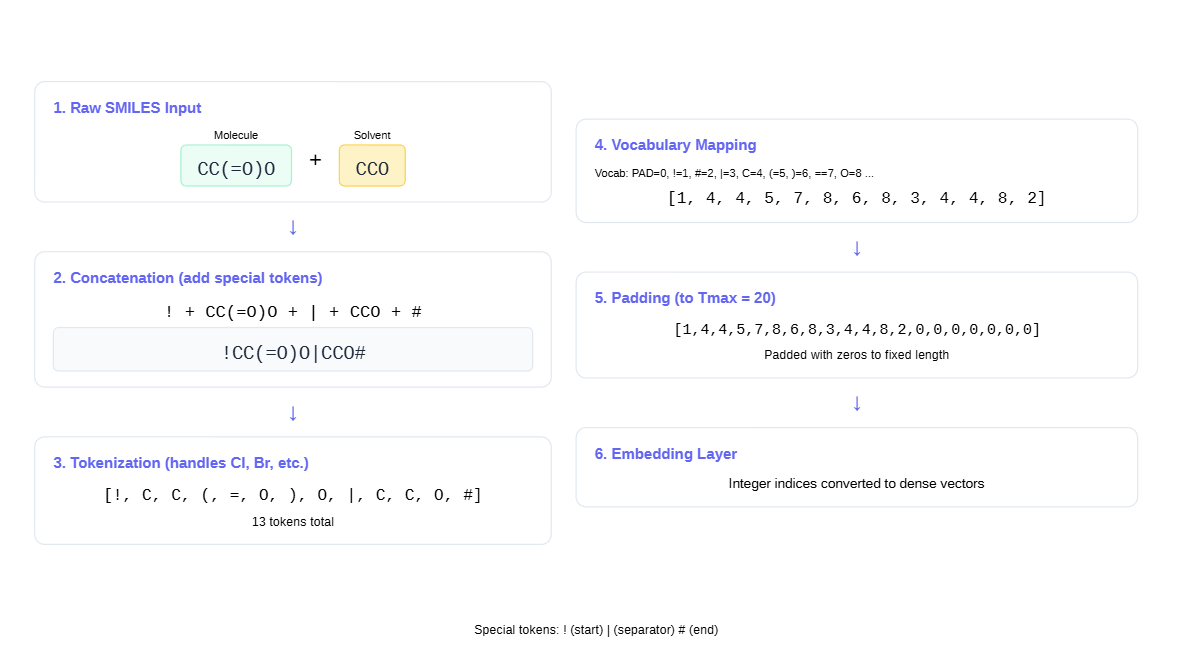
\includegraphics[width=\textwidth]{solvent_to_model.png}
    \caption{Molecule-Solvent concatenation example }
    \label{fig:example}
\end{figure}

The proposed concatenation strategy offers several advantages over alternative methods.

\paragraph{End-to-End Learning.} By encoding both solute and solvent within a single sequence, the model can learn representations that capture solute-solvent interactions directly from data without requiring explicit feature engineering. The recurrent architecture processes the concatenated sequence sequentially.

\paragraph{Unified Vocabulary.} Since both solute and solvent are represented using SMILES notation, they share a common tokenization vocabulary. This eliminates the need for separate encoding schemes and allows the embedding layer to learn unified representations of chemical tokens regardless of whether they appear in the solute or solvent context.



\section{Results and Discussion}

\subsection{RNN Model with SMILES Without Solvent Information}

The baseline model was trained using only canonical SMILES representations of the solute molecules, without any explicit encoding of solvent information. This approach treats UV absorption wavelength ($\lambda_{max}$) as an intrinsic molecular property, dependent solely on the electronic structure of the absorbing molecule.

\begin{figure}[H]
    \centering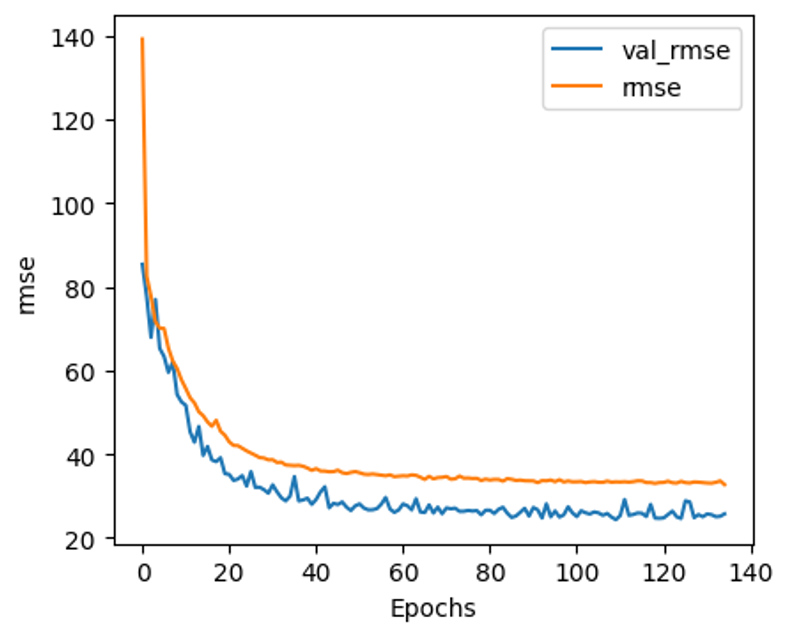
\includegraphics[scale=0.7]{canonwithoutsolvent.png}
    \caption{Training and validation RMSE as a function of epochs for the RNN model without solvent information. The model achieves convergence after approximately 130 epochs.}
    \label{fig:rmse_without_solvent}
\end{figure}

A minimum RMSE value of 24.36 nm was achieved after approximately 130 epochs.

While this baseline performance is reasonable, the RMSE of 24.36 nm indicates that relying solely on molecular structure has inherent limitations for predicting $\lambda_{max}$. This is expected from a theoretical standpoint, as solvatochromic effects shift in absorption wavelength due to solute-solvent interactions—are well-documented phenomena in spectroscopy \cite{reichardt2011solvents}. The magnitude of these shifts can range from a few to tens of nanometers, depending on the polarity and hydrogen-bonding characteristics of both the solute and solvent.

\subsection{RNN Model with SMILES and Solvent Information}

To address the limitations of the solvent-agnostic baseline, we implemented the concatenation strategy described, where SMILES representations of both the solute molecule and its corresponding solvent are combined into a single input sequence using special delimiter tokens. This approach enables the model to learn representations that capture solute-solvent interactions directly from the data.

\begin{figure}[H]
    \centering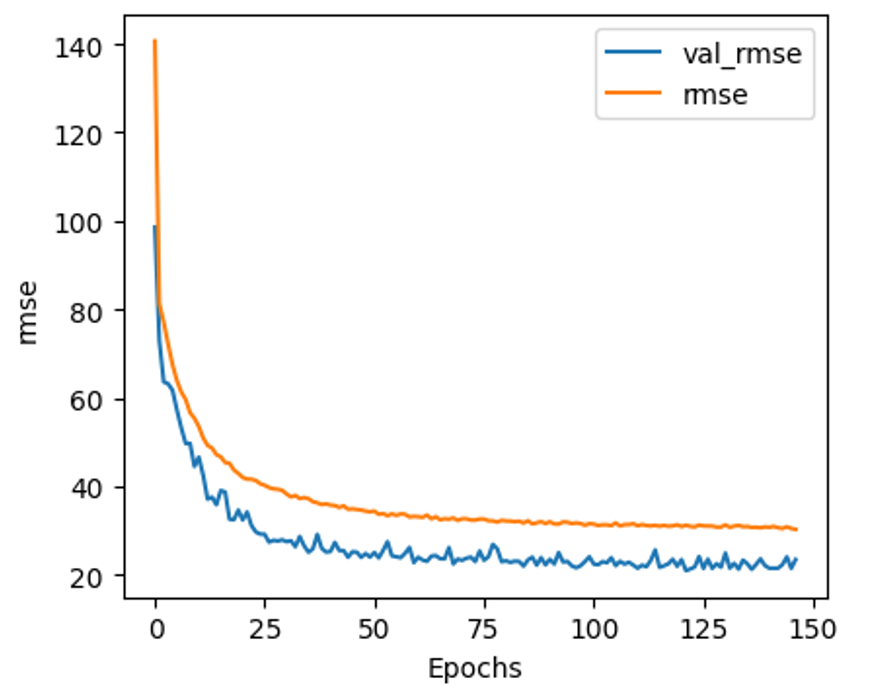
\includegraphics[scale=0.7]{canon1withsolvent.png}
    \caption{Training and validation RMSE as a function of epochs for the RNN model with solvent information incorporated via SMILES concatenation. The model achieves improved convergence with a lower minimum RMSE compared to the baseline.}
    \label{fig:rmse_with_solvent}
\end{figure}

Figure~\ref{fig:rmse_with_solvent} presents the learning curves for the solvent-aware model. The incorporation of solvent information substantially improved predictive performance, achieving a minimum RMSE of 20.34 nm after approximately 150 epochs. This represents a reduction of 4.02 nm on average (16.5\%) compared to the baseline model without solvent information.

% \subsubsection{Comparative Analysis and Discussion}

% Several key observations can be drawn from these results:

% \paragraph{Impact of Solvent Information.} The significant reduction in RMSE validates the importance of considering solute-solvent interactions for accurate $\lambda_{max}$ prediction. This finding aligns with established spectroscopic theory, where solvent polarity, hydrogen bonding capacity, and dielectric properties are known to influence electronic transition energies \cite{reichardt2011solvents, abraham1993scales}.

% \paragraph{Learning Dynamics.} The solvent-aware model required approximately 20 additional epochs to reach convergence compared to the baseline. This is expected, as the concatenated input sequences are longer and contain more complex patterns that the model must learn to interpret. The additional training time is a reasonable trade-off for the substantial improvement in predictive accuracy.

% \paragraph{Model Capacity.} The improvement demonstrates that the BiGRU architecture possesses sufficient capacity to learn meaningful representations from the concatenated SMILES sequences. The bidirectional processing allows information from both the solute and solvent portions to influence the final prediction, effectively capturing their interactions through the hidden state dynamics.

% \paragraph{Practical Implications.} From a practical standpoint, an RMSE of 20.34 nm is within a useful range for many pharmaceutical and chemical applications. For screening purposes, where the goal is to identify molecules with absorption in specific wavelength ranges (e.g., UVA, UVB, or visible), this level of accuracy can effectively prioritize candidates for experimental validation.

% \paragraph{Residual Error Sources.} The remaining prediction error may be attributed to several factors: (1) limitations in the SMILES representation, which does not explicitly encode three-dimensional conformational information; (2) the absence of concentration and temperature effects in the model; (3) potential noise or experimental uncertainty in the training data; and (4) complex multi-solvent or aggregation effects not captured by the simple concatenation approach.

% These results establish a strong foundation for the solvent-aware prediction framework and motivate further investigation into more sophisticated architectures and representation strategies.

%%%%%%%%%%%%%%%%%%%%%%%%%%%%%%%%%%%%%%%%%%%%%%%%%%%%%%%%%%%%%%%%%%%%%%%%%%%%%%%%%%%%%%%%%%%%%%%%%%%%%%%%%%

To further validate the model's predictive capability and assess its generalization to novel compounds, we conducted experimental UV-Vis spectroscopy measurements on a set of molecules not included in the training dataset. The experimentally determined $\lambda_{max}$ values were then compared against the model's predictions, as summarized in Table 2.1.
\begin{longtable}{|>{\raggedright\arraybackslash}p{4.2cm}|>{\centering\arraybackslash}p{3.5cm}|c|c|}
\caption{Input Molecules and the corresponding prediction of $\lambda_{\max}$ value against their experimental measurements in the solvent ethanol}
\label{tab:mytable} \\
\hline
\textbf{Molecule} & \textbf{Drawing of 2D Molecules} & \textbf{Exp $\lambda_{\max}$} & \textbf{Pred $\lambda_{\max}$} \\ \hline
\endfirsthead
\hline
\textbf{Molecule} & \textbf{Drawing of 2D Molecules} & \textbf{Exp $\lambda_{\max}$} & \textbf{Pred $\lambda_{\max}$} \\ \hline
\endhead
\hline
\endfoot
\textcolor{blue}{Avobenzone} \newline \texttt{\scriptsize O=C(c1ccc(cc1)C(C)(C)C)\allowbreak CC(=O)c2ccc(OC)cc2} & 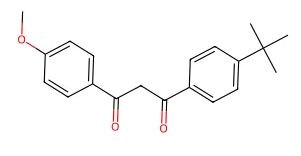
\includegraphics[width=3.3cm]{avobezone.png} & 358nm & 349nm\\ \hline
\textcolor{blue}{Ferulic Acid} \newline \texttt{\scriptsize COC1=C(C=CC(=C1)\allowbreak C=CC(=O)O)O} & 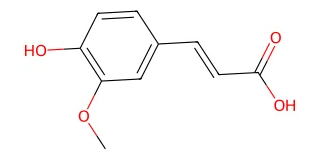
\includegraphics[width=3.3cm]{FerulicAcid.png} & 324nm & 335nm \\ \hline
\textcolor{blue}{Homosalate} \newline \texttt{\scriptsize O=C(OC1CC(CC(C1)(C)C)C)\allowbreak c2ccccc2O} & 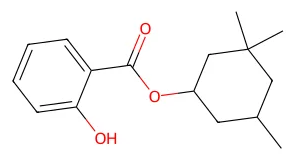
\includegraphics[width=3.3cm]{homosalate.png} & 308nm & 302nm\\ \hline
\textcolor{blue}{Octisalate} \newline \texttt{\scriptsize CCCCC(CC)COC(=O)\allowbreak C1=CC=CC=C1O} & 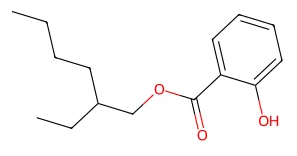
\includegraphics[width=3.3cm]{octisalate.png} & 308nm & 299nm\\ \hline
\textcolor{blue}{Oxybenzone} \newline \texttt{\scriptsize O=C(c1ccc(OC)cc1O)\allowbreak c2ccccc2} & 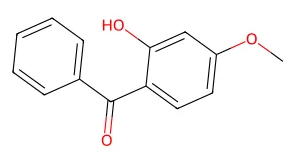
\includegraphics[width=3.3cm]{oxybenzone.png} & 287nm & 292nm \\ \hline
\end{longtable}


\section{Conclusion}

This work presented a sequential deep learning framework based on bidirectional GRU networks 
for predicting the maximum UV absorption wavelength ($\lambda_{\max}$) of organic molecules 
directly from their SMILES representations. By combining two large-scale experimental UV/Vis 
absorption databases totaling over 38,000 records, we assembled a chemically diverse training 
corpus spanning thousands of unique chromophores across hundreds of solvent conditions.

A central contribution of this work is the demonstration that incorporating solvent information 
via a simple yet effective SMILES concatenation strategy where solute and solvent 
representations are joined with special delimiter tokens into a single input sequence yields 
substantial improvements in prediction accuracy. The solvent-aware BiGRU model achieved an 
RMSE of 20.34~nm, a 16.5\% reduction compared to the solvent-agnostic baseline (RMSE = 
24.36~nm), confirming that solvent effects are a significant source of variability in 
$\lambda_{\max}$ that must be explicitly accounted for in predictive models.

Experimental validation on a set of commercially relevant UV-absorbing molecules---including 
avobenzone ($\Delta = 9$~nm), ferulic acid ($\Delta = 11$~nm), homosalate ($\Delta = 6$~nm), 
octisalate ($\Delta = 9$~nm), and oxybenzone ($\Delta = 5$~nm)---demonstrated that the model 
generalizes well to compounds outside the training distribution, with prediction errors consistent 
with the overall model RMSE.

The choice of RNN-based architectures over Transformer models was motivated by the local 
nature of UV absorption, which is primarily governed by chromophoric groups and their immediate 
electronic environments rather than long-range molecular dependencies. Empirical evidence from 
comparative studies supports that RNNs are well-suited for this property regime, particularly 
for moderate-length SMILES sequences typical of small to medium-sized organic chromophores.

Several directions for future work emerge from this study. First, the solvent encoding strategy 
could be extended to incorporate additional environmental parameters such as temperature, pH, 
and concentration. Second, attention mechanisms could be integrated into the BiGRU architecture 
to provide interpretability by identifying which molecular substructures contribute most to the 
predicted $\lambda_{\max}$, potentially offering chemical insight into structure-property 
relationships. Third, the trained prediction model serves as a natural component in a broader 
molecular design pipeline, specifically as a property filter within a Conditional Variational 
Autoencoder (CVAE) framework for the targeted generation of novel UV-absorbing molecules. 
Finally, expanding the training data to include computationally derived absorption spectra from 
time-dependent density functional theory (TD-DFT) calculations could further improve model 
coverage across underrepresented regions of chemical space.

In summary, this work demonstrates that sequential RNN deep networks with solvent-aware 
SMILES encoding provide an accurate, efficient, and practically deployable approach for 
predicting UV absorption properties, contributing to the accelerated computational design of 
UV-absorbing molecules for industrial and pharmaceutical applications.


\bibliographystyle{unsrtnat}
\bibliography{Proposal}

% ===== Supplementary Information =====

\end{document}
